\section{Shock wave simulation}
We studied the evolution of trans-relativistic shocks and spectum of accelerated particles. We chose relastivistic shocks with low lorentz-factor because the maximum energy of produced cosmic rays increases with shock wave lorentz-factor, but the efficiency of acceleration decreases, because it is more difficult for particle to cross fast moving front many times \cite{Ellison2013}. So we assume that intermediate case of trans-relativistic shocks provides the most effective acceleration.

We developed the implicit particle-in-cell (PIC) code, presented in our previous paper \cite{Romansky2016}, based on the scheme suggested by Lapenta et al.~\cite{Lapenta2006} and improved for the relativistic case by Noguchi et al.\cite{Noguchi2007}.
Our code is fully three dimensional and parallelized with MPI technology, which is adapted for distributed computing and can be executed on a wide class of computers.

In simulation setup the homogeneous plasma flows in through the right boundary
and collides with the reflecting superconducting wall on the left boundary, causing the shock wave. It is common way to initialize shock wave, because initialization using Rankine–Hugoniot conditions does not take in account microscopic distribution and shock wave, created that way, will probably fall apart for several discontinuities.
  
  Simulations are one-dimensional and have following parameters: initial flow lorentz-factor $\gamma = 1.5$, number densities $n_e = 10^{-4} \rm{cm}^{-3}$, $n_p = 10^{-4} \rm{cm}^{-3}$ , temperature $5\cdot10^8 \rm{K}$, magnetic field $B = 10^{-4} \rm{G}$, the full size of the box $L = 2\cdot10^{12} \rm{cm}$, the number of cells $N=2\cdot10^4$. Electron mass is reduced to $m_e = \frac{m_p}{20}$. The full time of simulation is $T = 5000 {\omega_p}^{-1}$. $\theta$ is angle between flow velocity and magnetic field. We present results of particle spectrum in several simulations with different $\theta$. 

\begin{figure}[h!]
	\centering
	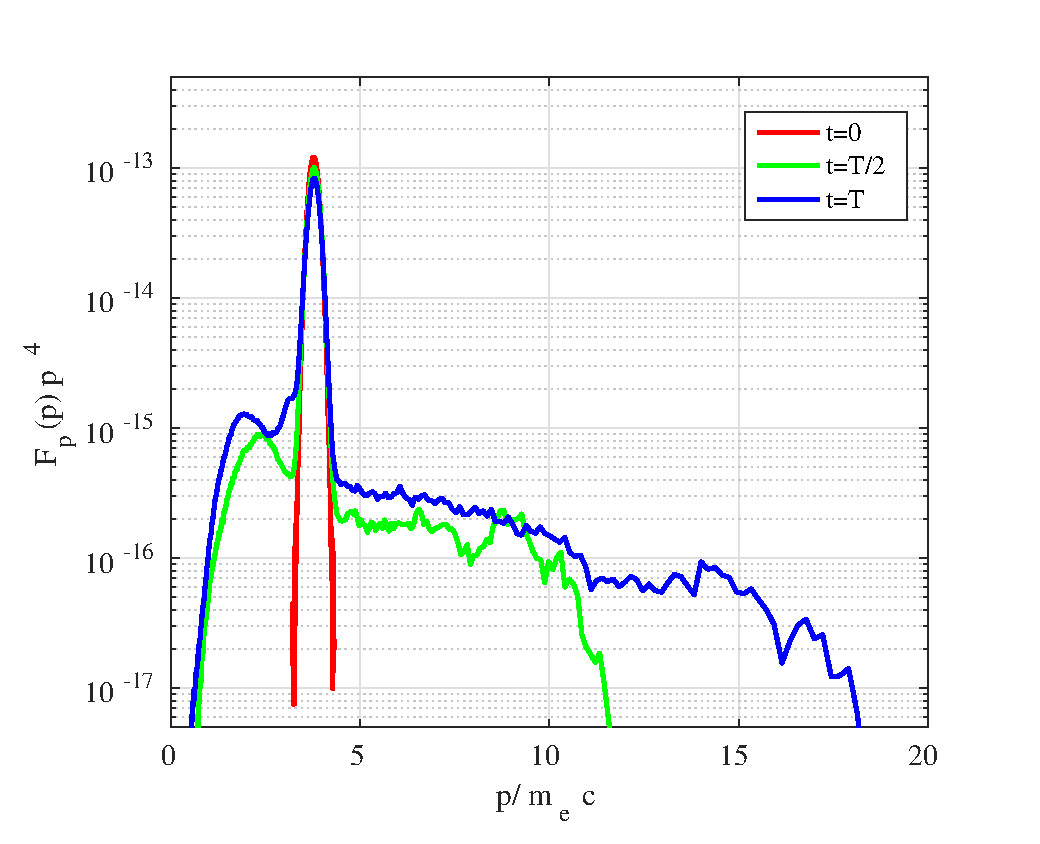
\includegraphics[width=0.95\textwidth]{fig/protons.eps} 
	\caption{Distribution of protons.}
	\label{protons}
\end{figure}
\begin{figure}[h!]
	\centering
	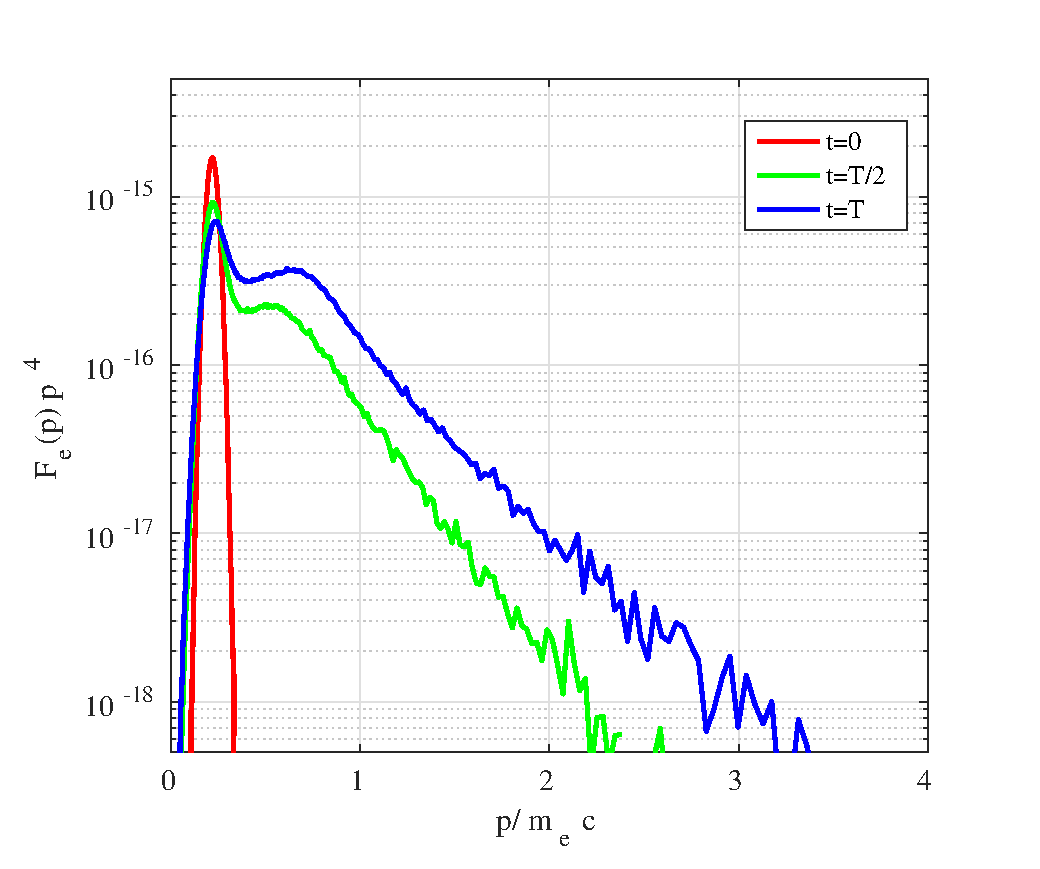
\includegraphics[width=0.95\textwidth]{fig/electrons.eps} 
	\caption{Distribution of electrons.}
	\label{electrons}
\end{figure}

One can see on Figures \ref{protons} and \ref{electrons} spectrum of particles with different angle $\theta$. Spectrum consists of three parts - narrow peak of cold but fast moving initial flow, wide peak of hot downstream and non-thermal accelerated component. Figures show that spectrum of accelerated particles strongly depends on angle $\theta$. If $\theta$ is less then critical value, defined by equation $c\cdot cos(\theta_{crit})=v_{shock}$, where all values are measured in upstream rest frame, particles can escape from the front and cross it several times to gain more energy. It is difficult to evaluate critical angle apriori, because we don't know compression relation of shock wave which will be created in simulation, but estimation for case of strong wave (compression relation $\sigma=4$) gets $\theta_{crit}=45^{\circ}$ in downstream frame. And it is consistent with results of our simulations.

Also, one can see that for angles less then critical, particle spectrum are higher and longer for larger $\theta$. Spectrum of nonthermal component is about 10 times higher for protons than for electrons at the same energy. It is consistent with other Particle-in-cell simulations o shock waves {\cite{Sironi2011}}.

Results show interesting effects for angles close to the critical value (black and yellow line)- electrons are still accelerating while protons are not. It can be explained by electrons accelerating in shortwave turbulence in precursor of shock wave.



